\documentclass{amsart}
\usepackage{etex}
\usepackage[T1]{fontenc}
\usepackage[utf8]{inputenx}

\title{The Rank 2 Roots Package \\ Version 1.0}
\author{Ben McKay}
\date{30 August 2018}

\usepackage{etoolbox} 
\usepackage{lmodern}
\usepackage[kerning=true,tracking=true]{microtype}
\usepackage{amsmath}
\usepackage{amsfonts}
\usepackage{array}
\usepackage{xparse}
\usepackage{xstring}
\usepackage{longtable}
\usepackage{rank-2-roots}
\usepackage{tikz}
\usepackage[listings]{tcolorbox} 
\tcbuselibrary{breakable}
\tcbuselibrary{skins}
\definecolor{example-color}{gray}{.85}
\definecolor{example-border-color}{gray}{.7} 
\tcbset{coltitle=black,colback=white,colframe=example-border-color,enhanced,breakable,pad at break*=1mm,
toprule=1.2mm,bottomrule=1.2mm,leftrule=1mm,rightrule=1mm,toprule at break=-1mm,bottomrule at break=-1mm,
before upper={\widowpenalties=3 10000 10000 150}}
\usepackage[pdftex]{hyperref}
\hypersetup{
  colorlinks   = true,  %Colours links instead of ugly boxes
  urlcolor     = black, %Colour for external hyperlinks
  linkcolor    = black, %Colour of internal links
  citecolor    = black  %Colour of citations
}
\usepackage{booktabs}
\usepackage{colortbl}
\usepackage{varwidth}
\usepackage{dynkin-diagrams}
\usepackage{fancyvrb}
\usepackage{xspace}
\newcommand{\TikZ}{Ti\textit{k}Z\xspace}
\usepackage{filecontents}
\usetikzlibrary{decorations.markings}
\usetikzlibrary{arrows,decorations.pathmorphing,backgrounds,positioning,fit}
\arrayrulecolor{white}
\makeatletter
    \def\rulecolor#1#{\CT@arc{#1}}
    \def\CT@arc#1#2{%
      \ifdim\baselineskip=\z@\noalign\fi
      {\gdef\CT@arc@{\color#1{#2}}}}
    \let\CT@arc@\relax
\rulecolor{white}
\makeatother





\NewDocumentCommand\todo{m}%
{%
\textcolor{blue}{\textit{#1}}
}%

\begin{document}
\maketitle
\tableofcontents

\section{Introduction}
This package concerns mathematical drawings arising in representation theory.
The purpose of this package is to ease drawing of rank 2 root systems, with Weyl chambers, weight lattices, and parabolic subgroups, mostly imitating the drawings of Fulton and Harris \cite{Fulton.Harris:1991}.
We use definitions of root systems and weight lattices as in Carter \cite{Carter:2005} p. 540--609.


\section{Root systems}
\NewDocumentCommand\drawroots{m}%
{%
\begin{tikzpicture}[baseline=-.5]
\begin{rootSystem}{#1}
\roots
\end{rootSystem}
\end{tikzpicture}
}%

\NewDocumentCommand\csdrawroots{m}%
{%
\texttt{\detokenize{\begin{tikzpicture}[baseline=-.5]}}%
\par\noindent%
\texttt{\detokenize{\begin{rootSystem}}\{#1\}}%
\par\noindent%
\texttt{\detokenize{\roots}}%
\par\noindent%
\texttt{\detokenize{\end{rootSystem}}}%
\par\noindent%
\texttt{\detokenize{\end{tikzpicture}}}%
}%

\newcommand*\mytablecontents{}
\foreach \i in {A,B,C,G}{
    \xappto\mytablecontents{$\i_2$ & \drawroots{\i} & \csdrawroots{\i}
}
  \gappto\mytablecontents{\\ \\}
}

\begin{longtable}{rcm{8cm}}
\caption{The root systems}\\
\endfirsthead
\caption{\dots continued}\\
\endhead
\multicolumn{3}{c}{continued \dots}\\
\endfoot
\endlastfoot
\mytablecontents
\end{longtable}


\section{Weights}
Type \verb!\wt{x}{y}! to get a weight at position \((x,y)\) (as measured in a basis of \emph{fundamental weights}).
Type \verb!\wt[multiplicity=n]{x}{y}! to get multiplicity \(m\).
Add an option: \verb!\wt[Z]{x}{y}{m}! to get \verb!Z! passed to TikZ.


\RenewDocumentCommand\drawroots{m}%
{%
\begin{tikzpicture}[baseline=-.5]
\begin{rootSystem}{#1}
\roots
\wt[brown]{1}{0}
\wt[red]{0}{1}
\wt[multiplicity=4,blue]{1}{3}
\wt[blue,multiplicity=2]{2}{2}
\wt[blue]{-1}{3}
\end{rootSystem}
\end{tikzpicture}
}%

\RenewDocumentCommand\csdrawroots{m}%
{%
\texttt{\detokenize{\begin{tikzpicture}[baseline=-.5]}}%
\par\noindent%
\texttt{\detokenize{\begin{rootSystem}}\{#1\}}%
\par\noindent%
\texttt{\detokenize{\roots}}%
\par\noindent%
\texttt{\detokenize{\wt[brown]{1}{0}}}%
\par\noindent%
\texttt{\detokenize{\wt[red]{0}{1}}}%
\par\noindent%
\texttt{\detokenize{\wt[multiplicity=4,blue]{1}{3}}}%
\par\noindent%
\texttt{\detokenize{\wt[blue,multiplicity=2]{2}{2}}}%
\par\noindent%
\texttt{\detokenize{\wt[blue]{-1}{3}}}%
\par\noindent%
\texttt{\detokenize{\end{rootSystem}}}%
\par\noindent%
\texttt{\detokenize{\end{tikzpicture}}}%
}%

\renewcommand*\mytablecontents{}
\foreach \i in {A,B,C,G}{
    \xappto\mytablecontents{$\i_2$ & \drawroots{\i} & \csdrawroots{\i}
}
  \gappto\mytablecontents{\\ \\}
}

\begin{longtable}{rcm{8cm}}
\caption{Some weights drawn with multiplicities}\\
\endfirsthead
\caption{\dots continued}\\
\endhead
\multicolumn{3}{c}{continued \dots}\\
\endfoot
\endlastfoot
\mytablecontents
\end{longtable}




\RenewDocumentCommand\drawroots{m}%
{%
\begin{tikzpicture}[baseline=-.5]
\begin{rootSystem}{#1}
\roots
\wt[multiplicity=2,root]{0}{0}
\end{rootSystem}
\end{tikzpicture}
}%

\RenewDocumentCommand\csdrawroots{m}%
{%
\texttt{\detokenize{\begin{tikzpicture}[baseline=-.5]}}%
\par\noindent%
\texttt{\detokenize{\begin{rootSystem}}\{#1\}}%
\par\noindent%
\texttt{\detokenize{\roots}}%
\par\noindent%
\texttt{\detokenize{\wt[multiplicity=2,root]{0}{0}}}%
\par\noindent%
\texttt{\detokenize{\end{rootSystem}}}%
\par\noindent%
\texttt{\detokenize{\end{tikzpicture}}}%
}%

\renewcommand*\mytablecontents{}
\foreach \i in {A,B,C,G}{
    \xappto\mytablecontents{$\i_2$ & \drawroots{\i} & \csdrawroots{\i}
}
  \gappto\mytablecontents{\\ \\}
}

\begin{longtable}{rcm{8cm}}
\caption{The root systems with all multiplicities of the adjoint representation, like Fulton and Harris}\\
\endfirsthead
\caption{\dots continued}\\
\endhead
\multicolumn{3}{c}{continued \dots}\\
\endfoot
\endlastfoot
\mytablecontents
\end{longtable}





















\RenewDocumentCommand\drawroots{m}%
{%
\begin{tikzpicture}[baseline=-.5]
\begin{rootSystem}{#1}
\roots
\WeylChamber
\end{rootSystem}
\end{tikzpicture}
}%

\RenewDocumentCommand\csdrawroots{m}%
{%
\texttt{\detokenize{\begin{tikzpicture}[baseline=-.5]}}%
\par\noindent%
\texttt{\detokenize{\begin{rootSystem}}\{#1\}}%
\par\noindent%
\texttt{\detokenize{\roots}}%
\par\noindent%
\texttt{\detokenize{\WeylChamber}}%
\par\noindent%
\texttt{\detokenize{\end{rootSystem}}}%
\par\noindent%
\texttt{\detokenize{\end{tikzpicture}}}%
}%

\renewcommand*\mytablecontents{}
\foreach \i in {A,B,C,G}{
    \xappto\mytablecontents{$\i_2$ & \drawroots{\i} & \csdrawroots{\i}
}
  \gappto\mytablecontents{\\ \\}
}

\begin{longtable}{rcm{8cm}}
\caption{Weyl chambers}\\
\endfirsthead
\caption{\dots continued}\\
\endhead
\multicolumn{3}{c}{continued \dots}\\
\endfoot
\endlastfoot
\mytablecontents
\end{longtable}




















\section{Parabolic subgroups}

\RenewDocumentCommand\drawroots{m}%
{%
\begin{tikzpicture}[baseline=-.5]
\begin{rootSystem}{#1}
\roots
\positiveRootHyperplane
\end{rootSystem}
\end{tikzpicture}
}%

\RenewDocumentCommand\csdrawroots{m}%
{%
\texttt{\detokenize{\begin{tikzpicture}[baseline=-.5]}}%
\par\noindent%
\texttt{\detokenize{\begin{rootSystem}}\{#1\}}%
\par\noindent%
\texttt{\detokenize{\roots}}%
\par\noindent%
\texttt{\detokenize{\positiveRootHyperplane}}%
\par\noindent%
\texttt{\detokenize{\end{rootSystem}}}%
\par\noindent%
\texttt{\detokenize{\end{tikzpicture}}}%
}%

\renewcommand*\mytablecontents{}
\foreach \i in {A,B,C,G}{
    \xappto\mytablecontents{$\i_2$ & \drawroots{\i} & \csdrawroots{\i}
}
  \gappto\mytablecontents{\\ \\}
}

\begin{longtable}{rcm{8cm}}
\caption{The positive root hyperplane}\\
\endfirsthead
\caption{\dots continued}\\
\endhead
\multicolumn{3}{c}{continued \dots}\\
\endfoot
\endlastfoot
\mytablecontents
\end{longtable}
























\RenewDocumentCommand\drawroots{mm}%
{%
\begin{tikzpicture}[baseline=-.5]
\begin{rootSystem}{#1}
\roots
\parabolic{#2}
\end{rootSystem}
\end{tikzpicture}
}%

\RenewDocumentCommand\csdrawroots{mm}%
{%
\texttt{\detokenize{\begin{tikzpicture}[baseline=-.5]}}%
\par\noindent%
\texttt{\detokenize{\begin{rootSystem}}\{#1\}}%
\par\noindent%
\texttt{\detokenize{\roots}}%
\par\noindent%
\texttt{\detokenize{\parabolic}\{#2\}}%
\par\noindent%
\texttt{\detokenize{\end{rootSystem}}}%
\par\noindent%
\texttt{\detokenize{\end{tikzpicture}}}%
}%

\renewcommand*\mytablecontents{}
\foreach \i in {A,B,C,G}{
	\foreach \j in {1,2,3}{
	    \xappto\mytablecontents{$\i_{2,\j}$ & \drawroots{\i}{\j} & \csdrawroots{\i}{\j}
	}
  \gappto\mytablecontents{\\ \\}
}
}

\begin{longtable}{rcm{8cm}}
\caption{Parabolic subgroups. Each set of roots is assigned a number, with each binary digit zero or one to say whether the corresponding root is crossed or not: \(A_{5,37}\) means the parabolic subgroup of \(A_5\) so that the binary digits of \(37=2^5+2^2+2^0\) give us roots \(0,2,5\) in Bourbaki ordering being compact roots, i.e. having the root vectors of both that root and its negative inside the parabolic subgroup. }\\
\endfirsthead
\caption{\dots continued}\\
\endhead
\multicolumn{3}{c}{continued \dots}\\
\endfoot
\endlastfoot
\mytablecontents
\end{longtable}



























\RenewDocumentCommand\drawroots{mm}%
{%
\begin{tikzpicture}[baseline=-.5]
\begin{rootSystem}{#1}
\roots
\parabolic{#2}
\parabolicgrading
\end{rootSystem}
\end{tikzpicture}
}%

\RenewDocumentCommand\csdrawroots{mm}%
{%
\texttt{\detokenize{\begin{tikzpicture}[baseline=-.5]}}%
\par\noindent%
\texttt{\detokenize{\begin{rootSystem}}\{#1\}}%
\par\noindent%
\texttt{\detokenize{\roots}}%
\par\noindent%
\texttt{\detokenize{\parabolic}\{#2\}}%
\par\noindent%
\texttt{\detokenize{\parabolicgrading}}%
\par\noindent%
\texttt{\detokenize{\end{rootSystem}}}%
\par\noindent%
\texttt{\detokenize{\end{tikzpicture}}}%
}%

\renewcommand*\mytablecontents{}
\foreach \i in {A,B,C,G}{
	\foreach \j in {1,2,3}{
	    \xappto\mytablecontents{$\i_{2,\j}$ & \drawroots{\i}{\j} & \csdrawroots{\i}{\j}
	}
  \gappto\mytablecontents{\\ \\}
}
}

\begin{longtable}{rcm{8cm}}
\caption{Parabolic subgroups with grading of the positive roots}\\
\endfirsthead
\caption{\dots continued}\\
\endhead
\multicolumn{3}{c}{continued \dots}\\
\endfoot
\endlastfoot
\mytablecontents
\end{longtable}




\NewDocumentCommand{\labelWt}{mmmm}%
{%
\node[#1,black] at \weight{#2}{#3} {\(#4\)};
}%


{
\NewDocumentCommand\labelRoots{}%
{%
\labelWt{above right}{0}{0}{0}%
\labelWt{right}{1}{1}{e_1-e_3}%
\labelWt{right}{2}{-1}{e_1-e_2}%
\labelWt{below}{1}{-2}{e_3-e_2}%
\labelWt{left}{-1}{-1}{e_3-e_1}%
\labelWt{left}{-2}{1}{e_2-e_1}%
\labelWt{above}{-1}{2}{e_2-e_3}%
}%
\setlength{\weightLength}{1cm}
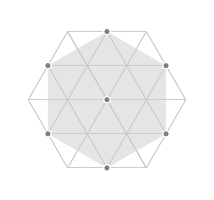
\begin{tikzpicture}
\begin{rootSystem}{A}
\roots
\wt{0}{0}
\labelRoots
\end{rootSystem}
\end{tikzpicture}
}


\tikzstyle{weight arrow}=[black,-stealth,shorten <=.25cm,shorten >=.25cm]

{
\NewDocumentCommand\wa{O{}mm}%
{%
\IfStrEq{#1}{0}%
{%
\draw[weight arrow]  \weight{#2}{#3} -- \weight{#2+1}{#3+1} node[right=-4pt]{\(0\)};%
}%
{%
\draw[weight arrow]  \weight{#2}{#3} -- \weight{#2+1}{#3+1};%
}%
}%
\setlength{\weightLength}{.75cm}
\begin{tikzpicture}
\begin{rootSystem}{A}
\setlength{\weightRadius}{1.5pt}
\roots
\wt{0}{0}
\labelWt{above left}{0}{0}{0}
\labelWt{right}{1}{1}{e_1-e_3}
\labelWt{right}{2}{-1}{e_1-e_2}
\labelWt{below}{1}{-2}{e_3-e_2}
\labelWt{left}{-1}{-1}{e_3-e_1}
\labelWt{left}{-2}{1}{e_2-e_1}
\labelWt{above left}{-1}{2}{e_2-e_3}
\wa{0}{0}
\wa[0]{1}{1}
\wa[0]{2}{-1}
\wa[0]{-1}{2}
\wa{1}{-2}
\wa{-1}{-1}
\wa{-2}{1}
\end{rootSystem}
\end{tikzpicture}
}



\begin{tcblisting}{title={Drawing the \(A_2\) root system and a weight at the origin. The option \texttt{root} indicates that this weight is to be coloured like a root.}}
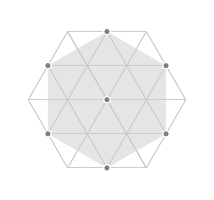
\begin{tikzpicture}
\begin{rootSystem}{A}
\roots
\wt[root]{0}{0}
\end{rootSystem}
\end{tikzpicture}
\end{tcblisting}


\begin{tcblisting}{title={Drawing the \(A_2\) root system and a weight at the origin and the positive root hyperplane}}
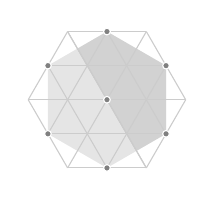
\begin{tikzpicture}
\begin{rootSystem}{A}
\roots
\wt[root]{0}{0}
\positiveRootHyperplane
\end{rootSystem}
\end{tikzpicture}
\end{tcblisting}




\section{Coordinate systems}

The package provides three coordinate systems: hex, square and weight.
Above we have seen the weight coordinates: a basis of fundamental weights.
We can also use weight coordinates like
\[
\verb!\draw \weight{0}{1} -- \weight{1}{0};!
\]
The square system, used like \verb!\draw (square cs:x=1,y=2) circle (2pt);!, is simply the standard Cartesian coordinate system measured so that the minimum distance between weights is one unit.
The hex coordinate system has basis precisely the fundamental weights of the \(A_2\) lattice.
We can use the hex system in drawing on the \(A_2\) or \(G_2\) weight lattices, as below, as they are the same lattices.

\begin{tcblisting}{title={Automatic sizing of the weight lattice (the default) \dots}}
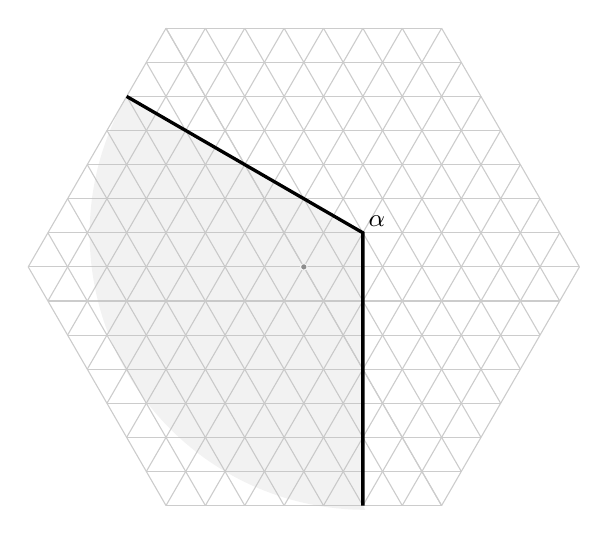
\begin{tikzpicture}
\begin{rootSystem}{A}
\wt{0}{0}
\fill[gray!50,opacity=.2]  (hex cs:x=5,y=-7) -- (hex cs:x=1,y=1) -- (hex cs:x=-7,y=5) arc (150:270:{7*\weightLength});
\draw[black,very thick] (hex cs:x=5,y=-7) -- (hex cs:x=1,y=1) -- (hex cs:x=-7,y=5);
\node[above right=-2pt] at (hex cs:x=1,y=1) {\small\(\alpha\)};
\end{rootSystem}
\end{tikzpicture}
\end{tcblisting}

\begin{tcblisting}{title={\dots and here with manual sizing, setting the weight lattice to include 3 steps to the right of the origin}}
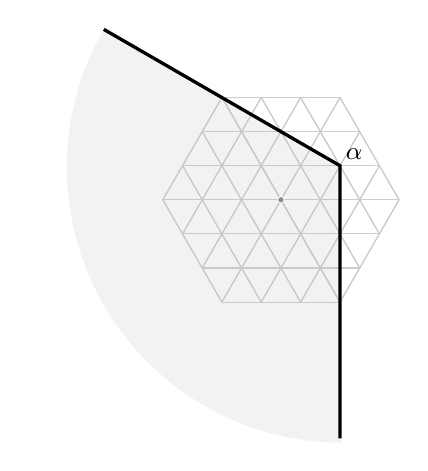
\begin{tikzpicture}
\AutoSizeWeightLatticefalse
\begin{rootSystem}{A}
\wt{0}{0}
\weightLattice{3}
\fill[gray!50,opacity=.2]  (hex cs:x=5,y=-7) -- (hex cs:x=1,y=1) -- (hex cs:x=-7,y=5) arc (150:270:{7*\weightLength});
\draw[black,very thick] (hex cs:x=5,y=-7) -- (hex cs:x=1,y=1) -- (hex cs:x=-7,y=5);
\node[above right=-2pt] at (hex cs:x=1,y=1) {\small\(\alpha\)};
\end{rootSystem}
\end{tikzpicture}
\end{tcblisting}

\begin{tcblisting}{title={Fulton and Harris p. 170}}
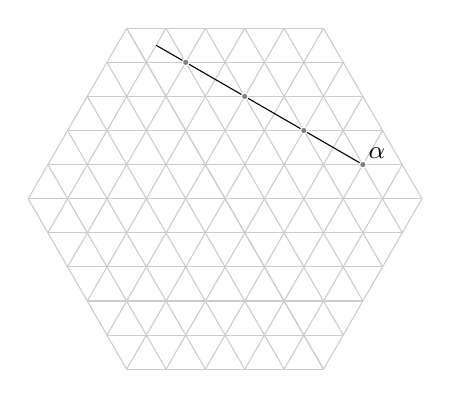
\begin{tikzpicture}
\begin{rootSystem}{A}
\draw \weight{3}{1} -- \weight{-4}{4.5};
\foreach \i in {1,...,4}{\wt{5-2*\i}{\i}}
\node[above right=-2pt] at (hex cs:x=3,y=1){\small\(\alpha\)};
\end{rootSystem}
\end{tikzpicture}
\end{tcblisting}





\begin{tcblisting}{title={Automatic sizing of the weight lattice (the default) \dots}}
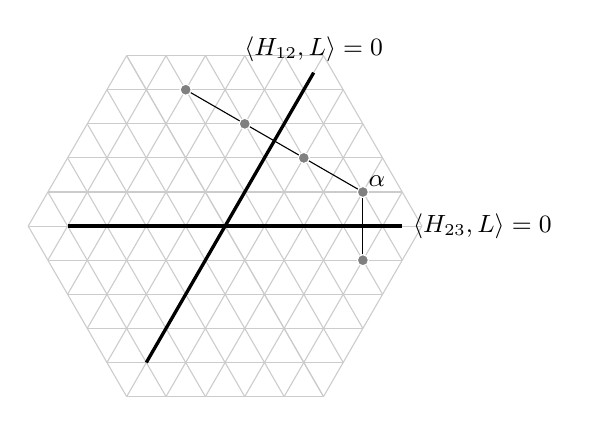
\begin{tikzpicture}
\begin{rootSystem}{A}
\setlength{\weightRadius}{2pt}
\draw \weight{3}{1} -- \weight{-3}{4};
\draw \weight{3}{1} -- \weight{4}{-1};
\wt{4}{-1}
\foreach \i in {1,...,4}{\wt{5-2*\i}{\i}}
\node[above right=-2pt] at (hex cs:x=3,y=1){\small\(\alpha\)};
\draw[very thick] \weight{0}{-4} -- \weight{0}{4.5} node[above]{\small\(\left<H_{12},L\right>=0\)};
\draw[very thick] \weight{-4}{0} -- \weight{4.5}{0} node[right]{\small\(\left<H_{23},L\right>=0\)};
\end{rootSystem}
\end{tikzpicture}
\end{tcblisting}


\begin{tcblisting}{title={\dots and manual sizing}}
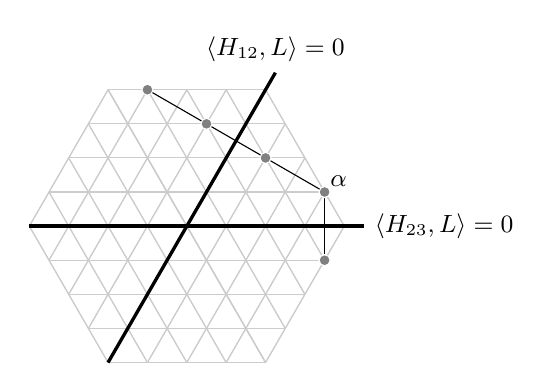
\begin{tikzpicture}
\AutoSizeWeightLatticefalse
\begin{rootSystem}{A}
\setlength{\weightRadius}{2pt}
\weightLattice{4}
\draw \weight{3}{1} -- \weight{-3}{4};
\draw \weight{3}{1} -- \weight{4}{-1};
\wt{4}{-1}
\foreach \i in {1,...,4}{\wt{5-2*\i}{\i}}
\node[above right=-2pt] at (hex cs:x=3,y=1){\small\(\alpha\)};
\draw[very thick] \weight{0}{-4} -- \weight{0}{4.5} node[above]{\small\(\left<H_{12},L\right>=0\)};
\draw[very thick] \weight{-4}{0} -- \weight{4.5}{0} node[right]{\small\(\left<H_{23},L\right>=0\)};
\end{rootSystem}
\end{tikzpicture}
\end{tcblisting}

\begin{tcblisting}{}
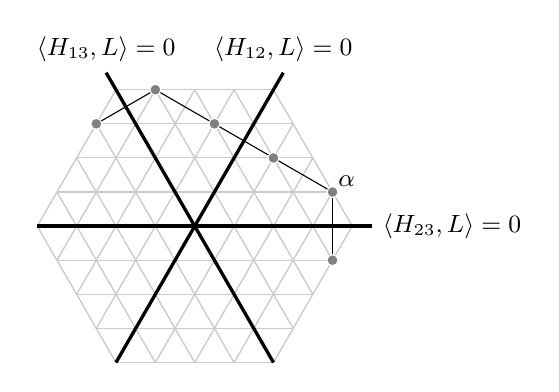
\begin{tikzpicture}
\AutoSizeWeightLatticefalse
\begin{rootSystem}{A}
\setlength{\weightRadius}{2pt}
\weightLattice{4}
\draw \weight{3}{1} -- \weight{-3}{4};
\draw \weight{3}{1} -- \weight{4}{-1};
\draw \weight{-3}{4} -- \weight{-4}{3};
\wt{4}{-1}
\wt{-4}{3}
\foreach \i in {1,...,4}{\wt{5-2*\i}{\i}}
\node[above right=-2pt] at (hex cs:x=3,y=1){\small\(\alpha\)};
\draw[very thick] \weight{0}{-4} -- \weight{0}{4.5} node[above]{\small\(\left<H_{12},L\right>=0\)};
\draw[very thick] \weight{-4}{0} -- \weight{4.5}{0} node[right]{\small\(\left<H_{23},L\right>=0\)};
\draw[very thick] \weight{4}{-4} -- \weight{-4.5}{4.5} node[above]{\small\(\left<H_{13},L\right>=0\)};
\end{rootSystem}
\end{tikzpicture}
\end{tcblisting}


\begin{tcblisting}{}
\setlength{\weightRadius}{2pt}
\setlength\weightLength{.75cm}
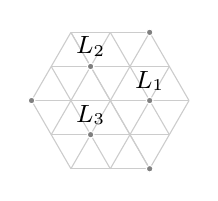
\begin{tikzpicture}
\begin{rootSystem}{A}
\foreach \x/\y in {1/0, -1/1, 0/-1, -2/0, 0/2, 2/-2}{\wt{\x}{\y}}
\node[above] at \weight{1}{0} {\small\(L_1\)};
\node[above] at \weight{-1}{1} {\small\(L_2\)};
\node[above] at \weight{0}{-1} {\small\(L_3\)};
\end{rootSystem}
\end{tikzpicture}
\end{tcblisting}

\begin{tcblisting}{title={Changing the weight length rescales}}

\begin{tikzpicture}
\setlength\weightLength{.3cm}
\begin{rootSystem}{A}
\wt[multiplicity=2]{0}{0}
\foreach \x/\y in {1/1, 2/-1, 1/-2, -1/-1, -2/1, -1/2}{\wt{\x}{\y}}
\end{rootSystem}
\end{tikzpicture}
\end{tcblisting}

\begin{tcblisting}{}
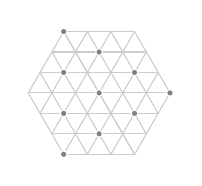
\begin{tikzpicture}
\setlength\weightLength{.3cm}
\begin{rootSystem}{A}
\foreach \x/\y in {0/0, 3/0, 2/-1, 1/-2, 0/-3, 1/1, -1/-1, -1/2, -2/1, -3/3}{\wt{\x}{\y}}
\end{rootSystem}
\end{tikzpicture}
\end{tcblisting}

\begin{tcblisting}{}
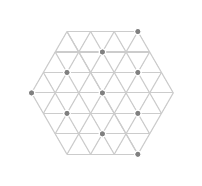
\begin{tikzpicture}
\setlength\weightLength{.3cm}
\begin{rootSystem}{A}
\foreach \x/\y in {0/0, -3/0, 2/-1, 1/-2, 3/-3, 1/1, -1/-1, -1/2, -2/1, 0/3}{\wt{\x}{\y}}
\end{rootSystem}
\end{tikzpicture}
\end{tcblisting}

\begin{tcblisting}{title={We use a basis of fundamental weights, as given in Carter's book \cite{Carter:2005} p. 540--609}}
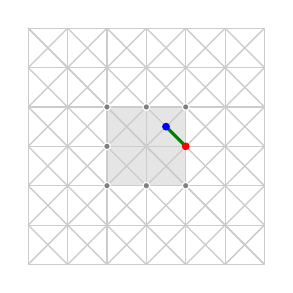
\begin{tikzpicture}
\begin{rootSystem}{B}
\roots
\draw[green!50!black,very thick] \weight{0}{1} -- \weight{1}{0};
\weightLattice{3}
\wt[blue]{1}{0}{1}
\wt[red]{0}{1}{1}
\end{rootSystem}
\end{tikzpicture}
\end{tcblisting}






Without automatic stretching of the weight lattice to fit the picture, you won't see the weight lattice at all unless you ask for it.

\AutoSizeWeightLatticefalse






\RenewDocumentCommand\drawroots{m}%
{%
\begin{tikzpicture}[baseline=-.5]
\begin{rootSystem}{#1}
\roots
\end{rootSystem}
\end{tikzpicture}
}%

\RenewDocumentCommand\csdrawroots{m}%
{%
\texttt{\detokenize{\begin{tikzpicture}[baseline=-.5]}}%
\par\noindent%
\texttt{\detokenize{\begin{rootSystem}}\{#1\}}%
\par\noindent%
\texttt{\detokenize{\roots}}%
\par\noindent%
\texttt{\detokenize{\end{rootSystem}}}%
\par\noindent%
\texttt{\detokenize{\end{tikzpicture}}}%
}%

\renewcommand*\mytablecontents{}
\foreach \i in {A,B,C,G}{
    \xappto\mytablecontents{$\i_2$ & \drawroots{\i} & \csdrawroots{\i}
}
  \gappto\mytablecontents{\\ \\}
}

\begin{longtable}{rcm{8cm}}
\caption{The root systems}\\
\endfirsthead
\caption{\dots continued}\\
\endhead
\multicolumn{3}{c}{continued \dots}\\
\endfoot
\endlastfoot
\mytablecontents
\end{longtable}




Type \verb!\wt{x}{y}{m}! to get a weight at position \((x,y)\) (as measured in a basis of \emph{fundamental weights}) with multiplicity \(m\).
Add an option: \verb!\wt[Z]{x}{y}{m}! to get \verb!Z! passed to TikZ.


\RenewDocumentCommand\drawroots{m}%
{%
\begin{tikzpicture}[baseline=-.5]
\begin{rootSystem}{#1}
\roots
\wt[brown]{1}{0}{1}
\wt[red]{0}{1}{1}
\wt[blue]{1}{3}{4}
\wt[blue]{2}{2}{2}
\wt[blue]{-1}{3}{1}
\end{rootSystem}
\end{tikzpicture}
}%

\RenewDocumentCommand\csdrawroots{m}%
{%
\texttt{\detokenize{\begin{tikzpicture}[baseline=-.5]}}%
\par\noindent%
\texttt{\detokenize{\begin{rootSystem}}\{#1\}}%
\par\noindent%
\texttt{\detokenize{\roots}}%
\par\noindent%
\texttt{\detokenize{\wt[brown]{1}{0}{1}}}%
\par\noindent%
\texttt{\detokenize{\wt[red]{0}{1}{1}}}%
\par\noindent%
\texttt{\detokenize{\wt[blue]{1}{3}{4}}}%
\par\noindent%
\texttt{\detokenize{\wt[blue]{2}{2}{2}}}%
\par\noindent%
\texttt{\detokenize{\wt[blue]{-1}{3}{1}}}%
\par\noindent%
\texttt{\detokenize{\end{rootSystem}}}%
\par\noindent%
\texttt{\detokenize{\end{tikzpicture}}}%
}%

\renewcommand*\mytablecontents{}
\foreach \i in {A,B,C,G}{
    \xappto\mytablecontents{$\i_2$ & \drawroots{\i} & \csdrawroots{\i}
}
  \gappto\mytablecontents{\\ \\}
}

\begin{longtable}{rcm{8cm}}
\caption{Some weights drawn with multiplicities}\\
\endfirsthead
\caption{\dots continued}\\
\endhead
\multicolumn{3}{c}{continued \dots}\\
\endfoot
\endlastfoot
\mytablecontents
\end{longtable}




\RenewDocumentCommand\drawroots{m}%
{%
\begin{tikzpicture}[baseline=-.5]
\begin{rootSystem}{#1}
\roots
\wt[multiplicity=2]{0}{0}
\end{rootSystem}
\end{tikzpicture}
}%

\RenewDocumentCommand\csdrawroots{m}%
{%
\texttt{\detokenize{\begin{tikzpicture}[baseline=-.5]}}%
\par\noindent%
\texttt{\detokenize{\begin{rootSystem}}\{#1\}}%
\par\noindent%
\texttt{\detokenize{\roots}}%
\par\noindent%
\texttt{\detokenize{\wt[multiplicity=2]{0}{0}}}%
\par\noindent%
\texttt{\detokenize{\end{rootSystem}}}%
\par\noindent%
\texttt{\detokenize{\end{tikzpicture}}}%
}%

\renewcommand*\mytablecontents{}
\foreach \i in {A,B,C,G}{
    \xappto\mytablecontents{$\i_2$ & \drawroots{\i} & \csdrawroots{\i}
}
  \gappto\mytablecontents{\\ \\}
}

\begin{longtable}{rcm{8cm}}
\caption{The root systems with all multiplicities of the adjoint representation, like Fulton and Harris}\\
\endfirsthead
\caption{\dots continued}\\
\endhead
\multicolumn{3}{c}{continued \dots}\\
\endfoot
\endlastfoot
\mytablecontents
\end{longtable}





















\RenewDocumentCommand\drawroots{m}%
{%
\begin{tikzpicture}[baseline=-.5]
\begin{rootSystem}{#1}
\roots
\WeylChamber
\end{rootSystem}
\end{tikzpicture}
}%

\RenewDocumentCommand\csdrawroots{m}%
{%
\texttt{\detokenize{\begin{tikzpicture}[baseline=-.5]}}%
\par\noindent%
\texttt{\detokenize{\begin{rootSystem}}\{#1\}}%
\par\noindent%
\texttt{\detokenize{\roots}}%
\par\noindent%
\texttt{\detokenize{\WeylChamber}}%
\par\noindent%
\texttt{\detokenize{\end{rootSystem}}}%
\par\noindent%
\texttt{\detokenize{\end{tikzpicture}}}%
}%

\renewcommand*\mytablecontents{}
\foreach \i in {A,B,C,G}{
    \xappto\mytablecontents{$\i_2$ & \drawroots{\i} & \csdrawroots{\i}
}
  \gappto\mytablecontents{\\ \\}
}

\begin{longtable}{rcm{8cm}}
\caption{Weyl chambers}\\
\endfirsthead
\caption{\dots continued}\\
\endhead
\multicolumn{3}{c}{continued \dots}\\
\endfoot
\endlastfoot
\mytablecontents
\end{longtable}



























\RenewDocumentCommand\drawroots{m}%
{%
\begin{tikzpicture}[baseline=-.5]
\begin{rootSystem}{#1}
\roots
\positiveRootHyperplane
\end{rootSystem}
\end{tikzpicture}
}%

\RenewDocumentCommand\csdrawroots{m}%
{%
\texttt{\detokenize{\begin{tikzpicture}[baseline=-.5]}}%
\par\noindent%
\texttt{\detokenize{\begin{rootSystem}}\{#1\}}%
\par\noindent%
\texttt{\detokenize{\roots}}%
\par\noindent%
\texttt{\detokenize{\positiveRootHyperplane}}%
\par\noindent%
\texttt{\detokenize{\end{rootSystem}}}%
\par\noindent%
\texttt{\detokenize{\end{tikzpicture}}}%
}%

\renewcommand*\mytablecontents{}
\foreach \i in {A,B,C,G}{
    \xappto\mytablecontents{$\i_2$ & \drawroots{\i} & \csdrawroots{\i}
}
  \gappto\mytablecontents{\\ \\}
}

\begin{longtable}{rcm{8cm}}
\caption{The positive root hyperplane}\\
\endfirsthead
\caption{\dots continued}\\
\endhead
\multicolumn{3}{c}{continued \dots}\\
\endfoot
\endlastfoot
\mytablecontents
\end{longtable}
























\RenewDocumentCommand\drawroots{mm}%
{%
\begin{tikzpicture}[baseline=-.5]
\begin{rootSystem}{#1}
\roots
\parabolic{#2}
\end{rootSystem}
\end{tikzpicture}
}%

\RenewDocumentCommand\csdrawroots{mm}%
{%
\texttt{\detokenize{\begin{tikzpicture}[baseline=-.5]}}%
\par\noindent%
\texttt{\detokenize{\begin{rootSystem}}\{#1\}}%
\par\noindent%
\texttt{\detokenize{\roots}}%
\par\noindent%
\texttt{\detokenize{\parabolic}\{#2\}}%
\par\noindent%
\texttt{\detokenize{\end{rootSystem}}}%
\par\noindent%
\texttt{\detokenize{\end{tikzpicture}}}%
}%

\renewcommand*\mytablecontents{}
\foreach \i in {A,B,C,G}{
	\foreach \j in {1,2,3}{
	    \xappto\mytablecontents{$\i_{2,\j}$ & \drawroots{\i}{\j} & \csdrawroots{\i}{\j}
	}
  \gappto\mytablecontents{\\ \\}
}
}

\begin{longtable}{rcm{8cm}}
\caption{Parabolic subgroups}\\
\endfirsthead
\caption{\dots continued}\\
\endhead
\multicolumn{3}{c}{continued \dots}\\
\endfoot
\endlastfoot
\mytablecontents
\end{longtable}



























\RenewDocumentCommand\drawroots{mm}%
{%
\begin{tikzpicture}[baseline=-.5]
\begin{rootSystem}{#1}
\roots
\parabolic{#2}
\parabolicgrading
\end{rootSystem}
\end{tikzpicture}
}%

\RenewDocumentCommand\csdrawroots{mm}%
{%
\texttt{\detokenize{\begin{tikzpicture}[baseline=-.5]}}%
\par\noindent%
\texttt{\detokenize{\begin{rootSystem}}\{#1\}}%
\par\noindent%
\texttt{\detokenize{\roots}}%
\par\noindent%
\texttt{\detokenize{\parabolic}\{#2\}}%
\par\noindent%
\texttt{\detokenize{\parabolicgrading}}%
\par\noindent%
\texttt{\detokenize{\end{rootSystem}}}%
\par\noindent%
\texttt{\detokenize{\end{tikzpicture}}}%
}%

\renewcommand*\mytablecontents{}
\foreach \i in {A,B,C,G}{
	\foreach \j in {1,2,3}{
	    \xappto\mytablecontents{$\i_{2,\j}$ & \drawroots{\i}{\j} & \csdrawroots{\i}{\j}
	}
  \gappto\mytablecontents{\\ \\}
}
}

\begin{longtable}{rcm{8cm}}
\caption{Parabolic subgroups with grading of the positive roots}\\
\endfirsthead
\caption{\dots continued}\\
\endhead
\multicolumn{3}{c}{continued \dots}\\
\endfoot
\endlastfoot
\mytablecontents
\end{longtable}





\section{Examples of weights of various representations}

Henceforth assume \verb!\AutoSizeWeightLatticetrue! (the default).

\AutoSizeWeightLatticetrue


\begin{tcblisting}{title={Fulton and Harris, p. 186}}
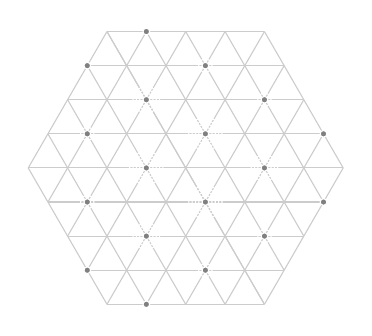
\begin{tikzpicture}
\begin{rootSystem}{A}
\foreach \x/\y/\m in 
{0/ 1/5,  -1/0/5,  1/-1/5,  2/ 0/4, -2/ 2/4,  0/-2/4, 
 1/ 2/2,  -1/3/2,  3/-2/2,  2/-3/2, -2/-1/2, -3/ 1/2,
 4/-1/1,   3/1/1, -3/ 4/1, -4/ 3/1, -1/-3/1,  1/-4/1}
{\wt[multiplicity=\m]{\x}{\y}}
\end{rootSystem}
\end{tikzpicture}
\end{tcblisting}


\begin{tcblisting}{title={A representation of \(G_2\)}}
\setlength\weightLength{1cm}
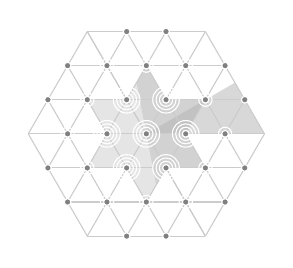
\begin{tikzpicture}
\begin{rootSystem}{G}
\roots
\foreach \m/\x/\y in {
1/1/1, 1/4/-1, 1/-1/2, 2/2/0, 1/5/-2,
2/0/1, 2/3/-1, 2/-2/2, 4/1/0, 1/-4/3,
2/4/-2, 4/-1/1, 4/2/-1,  2/-3/2, 1/5/-3,
4/0/0, 1/-5/3, 2/3/-2, 4/-2/1, 4/1/-1,
2/-4/2, 1/4/-3, 4/-1/0, 2/2/-2, 2/-3/1, 
2/0/-1, 1/-5/2, 2/-2/0, 1/1/-2, 1/-4/1,
1/-1/-1}{\wt[multiplicity=\m]{\x}{\y}}
\positiveRootHyperplane
\WeylChamber
\end{rootSystem}
\end{tikzpicture}
\end{tcblisting}


\begin{tcblisting}{title={Dimensions of representations of \(G_2\), parameterized by highest weight}}
\setlength\weightLength{1cm}
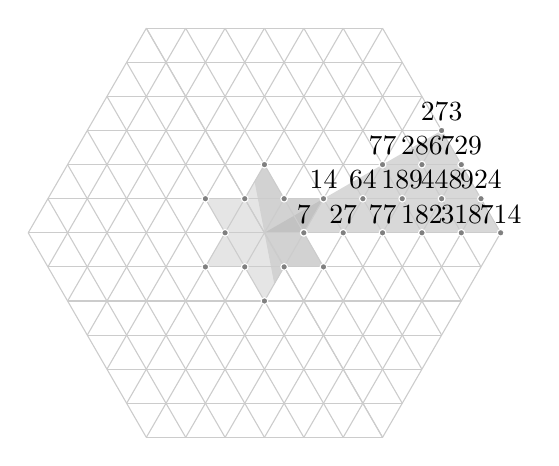
\begin{tikzpicture}
\begin{rootSystem}{G}
\roots
\foreach \x/\y/\d in {
0/1/14, 0/2/77, 0/3/273, 1/0/7, 1/1/64,
1/2/286, 2/0/27, 2/1/189, 2/2/729, 3/0/77,
4/0/182, 5/0/318, 6/0/714, 3/1/448, 4/1/924}
{\wt{\x}{\y}\node[black,above] at \weight{\x}{\y} {\(\d\)};}
\positiveRootHyperplane
\WeylChamber
\end{rootSystem}
\end{tikzpicture}
\end{tcblisting}


\bibliographystyle{amsplain}
\bibliography{rank-2-roots}

\end{document}
